\section{Framework Concept}

\subsection{Introduction}

In this chapter, the general concept of the Golem network architecture will be presented. 
Both the assumptions and elements of the network, applications, services, protocols will be 
described in the most abstract way possible, so as not to lose the idea of ​​solving the system 
due to the complexity of the processes taking place in it.

A detailed description of the components will be described later in the document.

\subsection{Definitions}

\begin{description}

\item[Plane] This is a set of elements (physical, virtual or their abstractions),
applications, services, protocols, functions that allow for internal
and external communication, their configuration and monitoring at all layers.

\end{description}

\subsection{Abstract Architecture}

The architecture of the Golem Network will be presented on three planes 
(Please see Figure ~\ref{fig:Plane} on page ~\pageref{fig:Plane}):

\begin{enumerate}
	\item Golem Plane (GP)
	\item User Plane (UP)
	\item External Provider Plane (EPP)
\end{enumerate}

\begin{figure}[htbp]
    \centering
    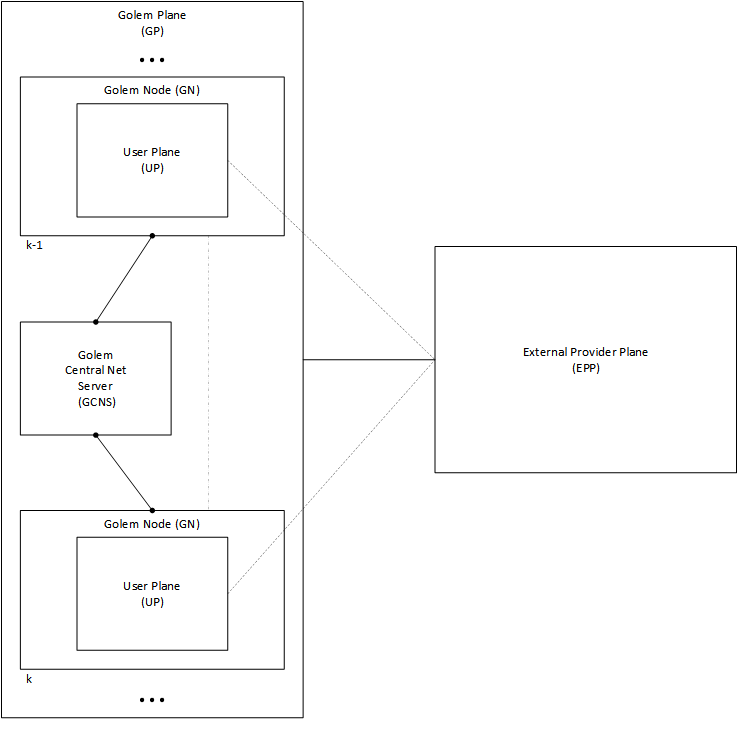
\includegraphics[width=7cm,height=7cm,angle=0]{./diag/03.AbsPlane-Diag-v002.png}
    \caption{Abstraction Plane Concept}
	\label{fig:Plane}
\end{figure}

The Golem Plane is the basis on which nodes called Golem Nodes are defined, 
which together with the Central Net Server build the Golem Network 
(Please see Figure ~\ref{fig:Ntw} on page ~\pageref{fig:Ntw}).

\begin{figure}[htbp]
    \centering
    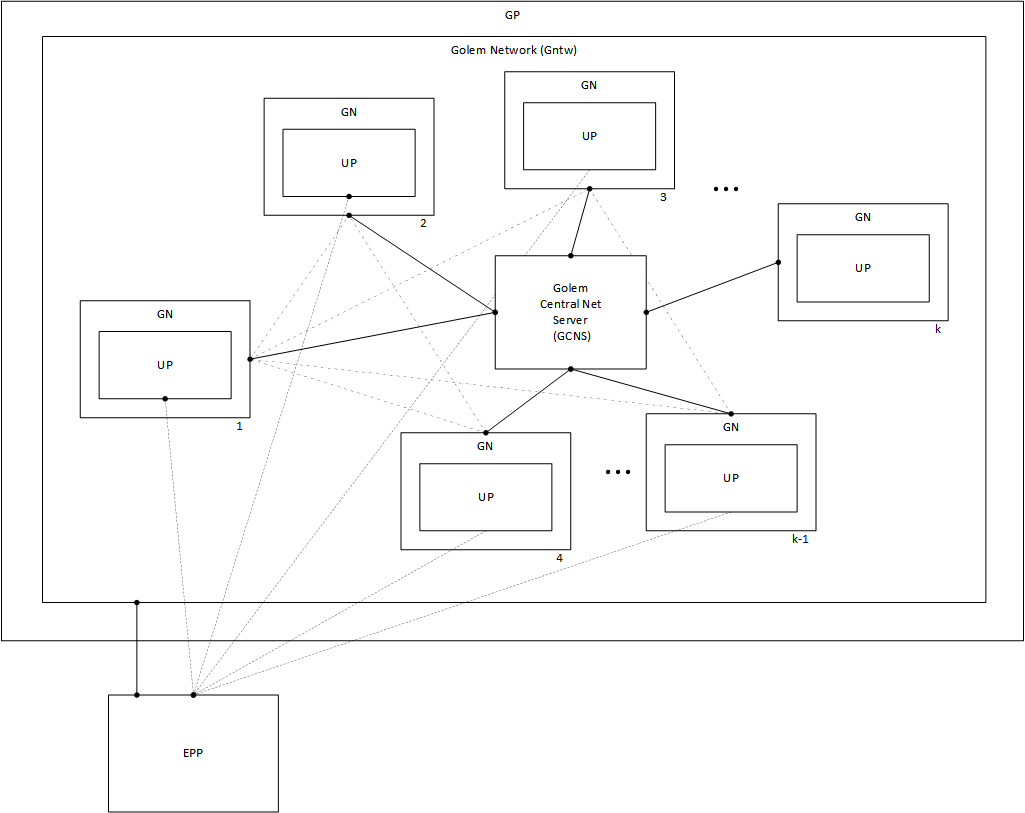
\includegraphics[width=7cm,height=7cm,angle=0]{./diag/02.AbsNtw-Diag-v002.png}
	\caption{Abstraction Network Concept}
    \label{fig:Ntw}
\end{figure}

Each node consists of a set of core applications, core services
and core protocols enabling communication, configuration and monitoring 
on all layers of decentralized and distributed business processes.
Business processes are implemented on the User Plane using functions of 
core components of applications, services and protocols through their API.
The External Operator Plane is used for specific functions implemented
outside the Golem Network but used by this network. An example is the availability of
payments in cryptocurrencies.

The above Planes with their component elements distributed over three main layers 
are shown in the figure 
(Please see Figure ~\ref{fig:Arch} on page ~\pageref{fig:Arch}):

\begin{enumerate}
	\item Platform Layer (PL)
	\item Integration Layer (IL)
	\item Application and Services Layer (ASL)
\end{enumerate}

\afterpage{
\begin{landscape}
	\begin{figure}[htbp]
		\centering
		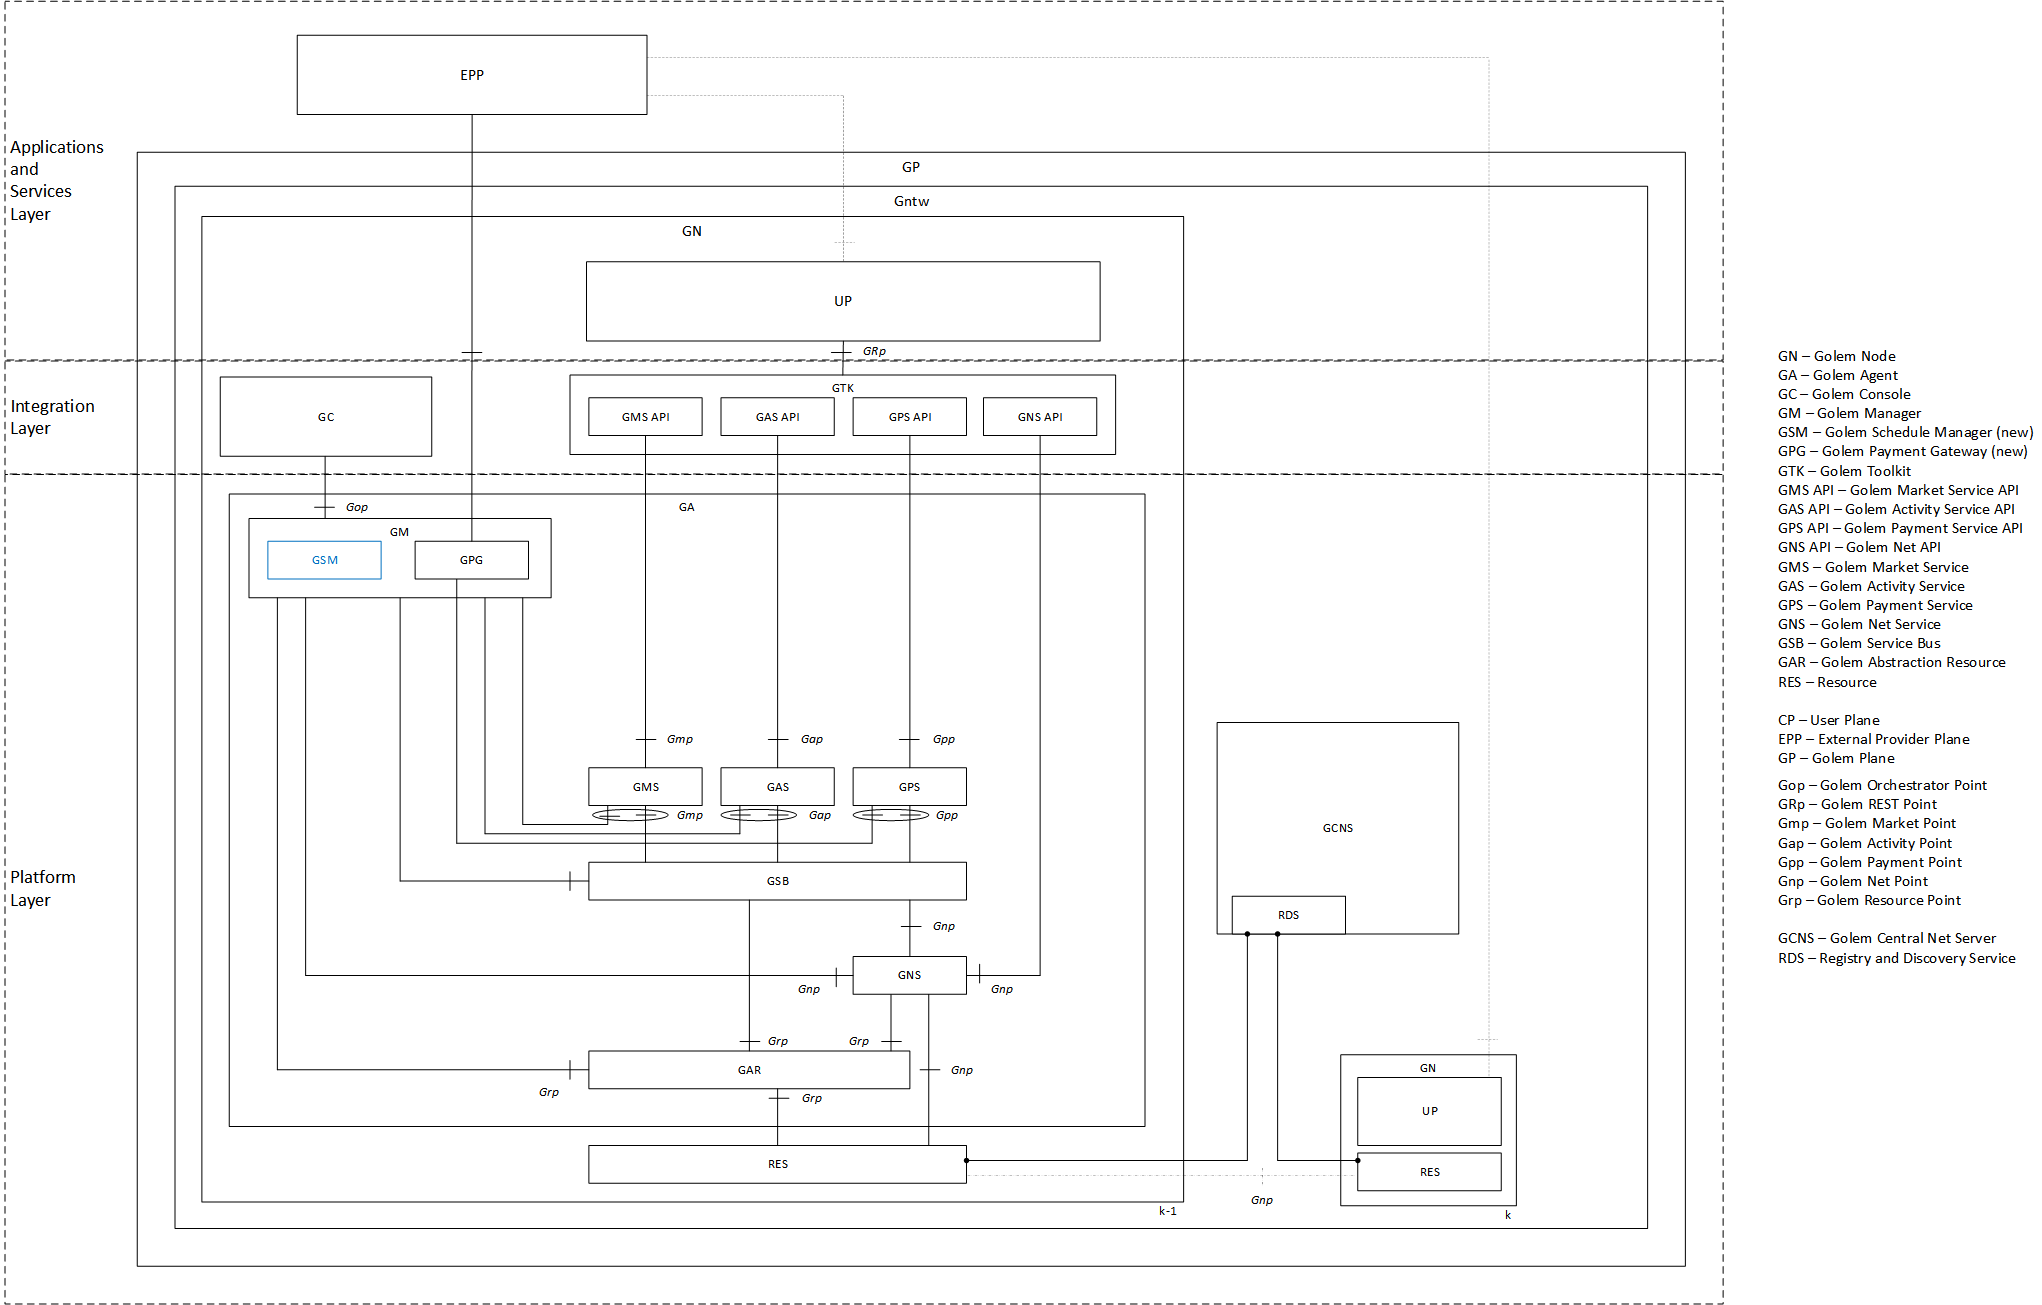
\includegraphics[width=\hsize]{./diag/01.AbsArch-Diag-v002.png}
		\caption{Abstraction Architecture Diagram}
		\label{fig:Arch}
	\end{figure}
\end{landscape}
}

In the Platform Layer there is the Golem Agent (GA) element, which allows to create a Golem Node (GN) from a computer unit, 
which is a member of the Golem network (Gntw).

In the Integration Layer there is the Golem Agent Console (GAC) and the Golem Toolkit (GTK). 
The Golem Agent Console consists of tools for configuring and monitoring created applications and services 
and managing the Golem Agent element, which is the daemon of the created node (GN). 
The Golem Toolkit is a set of tools, APIs, which allow to create decentralized and distributed applications and services
on the Golem network infrastructure.

In the Applications and Services Layer there is the User Plane (UP) and the External Provider Plane (EPP).

On the User Plane, decentralized applications and services of the Golem network Users are implemented,
which can use service and application templates created in the form of a "standards - change the name" specification framework.

On this plane, user roles are defined, which can be assigned to Golem Nodes depending on the aspect of the node's computational resources and/or the service it provides.
A single aspect of a resource and/or service defines a dimension of the namespace.
Thus, a set of dimensions creates a multidimensional structure of the namespace.

Golem Agent contains basic tools for creating a decentralized market of distributed applications and services.
These are:

\begin{enumerate}

\item {\bf Golem Market Service (GMS)}

This service has functions for creating a market of distributed computing resources.
This service allows sellers (Providers) to describe the subject of sale in the form of an offer
and buyers (Requestors) to describe the subject of demand in the form of a Demand.
The basic elements of the offer are:


\begin{itemize}
\item	Resource Vector
\item  	Usage Vector
\item  	Context Vector
\item 	Pricing Function
\end{itemize}

In addition, the service allows for decentralized searches of offers and demands in order to associate them
based on the conditions described in offers and demands. Matched objects are represented as
proposal. An accepted and confirmed proposal allows for the creation of an agreement object, which
after being signed by the parties is a confirmation of the sale and purchase of goods such as computing resources.

The Market service is based on the tuple space (Tuples Space).
A tuple is a finite list of elements that can be used to represent a data item or a message.

In the Golem system, in the Market service, tuples are used to describe objects such as:
offer, demand, proposal, agreement. The space is used to define interaction functions on these objects
such as:

\begin{itemize}
\item  Observation
\item  Discovery
\item  Negotiation
\item  Agreement
\end{itemize}

\item {\bf Golem Activity Service (GAS)}

This service has tools that allow the Requestor's applications and services to be launched on the Provider's computing resources,
while simultaneously measuring the use of these resources in accordance with the concluded contract in the form of an agreement. The measurement of the use of
resources is recorded in the form of metrics in the Usage Counters Vector (UCV) object.

\item {\bf Golem Payment Service (GPS)}

This service enables settlements between the parties based on the terms contained in the contract. Usage Counters Vector (UCV) objects created in the Golem Activity Service and the settlement terms included in the agreement are used to settle the sale-purchase item.

The Usage Counters Vector (UCV) associated with the agreement and activity creates Activity Detail Record (ADR) objects.

Settlement functions allow the ADR object to be transformed into a Debit Note (DN) object, where the total incremental settlement amounts for using Provider resources are included. The frequency of creating and sending Debit Notes objects between the parties is included in the agreement. The state of completing the use of Provider resources allows for the generation of an invoice summarizing the agreement between the parties. Payment is made via the blockchain operator. Optimization of payment transaction costs is
possible by setting the terms of this operation in the agreement object.

\item {\bf Golem Net Service (GNS)}

In a single node, the above services communicate with each other via the Golem Service Bus (GSB).

In turn, communication between nodes takes place via the Golem Net Service (GNS) service, which provides peer to peer (p2p) protocols.

This service also provides communication to the Registry and Discovery Service located on the Golem Central Net Server (GCNS).

\item {\bf Golem Services API}

The following APIs are available:

\begin{itemize}
\item Golem Market Service API (GMS API)
\item Golem Activity Service API (GAS API)
\item Golem Payment Service API (GPS API)
\item Golem Net Service API (GNS API)
\item Golem Service Bus API (GSB API)
\end{itemize}

All of the above services have APIs that allow you to create new decentralized and distributed applications and services,
which use the created Golem network infrastructure (Gntw) and the genericity properties of the underlying services.

The APIs of individual services also allow you to create interaction automation, e.g. settlements, 
and offer optimization and orders, and many other tools.

\end{enumerate}



\break

\subsection{Reference Architecture}